\documentclass{standalone}
\usepackage{tikz}
\usetikzlibrary{patterns, positioning}


\begin{document}
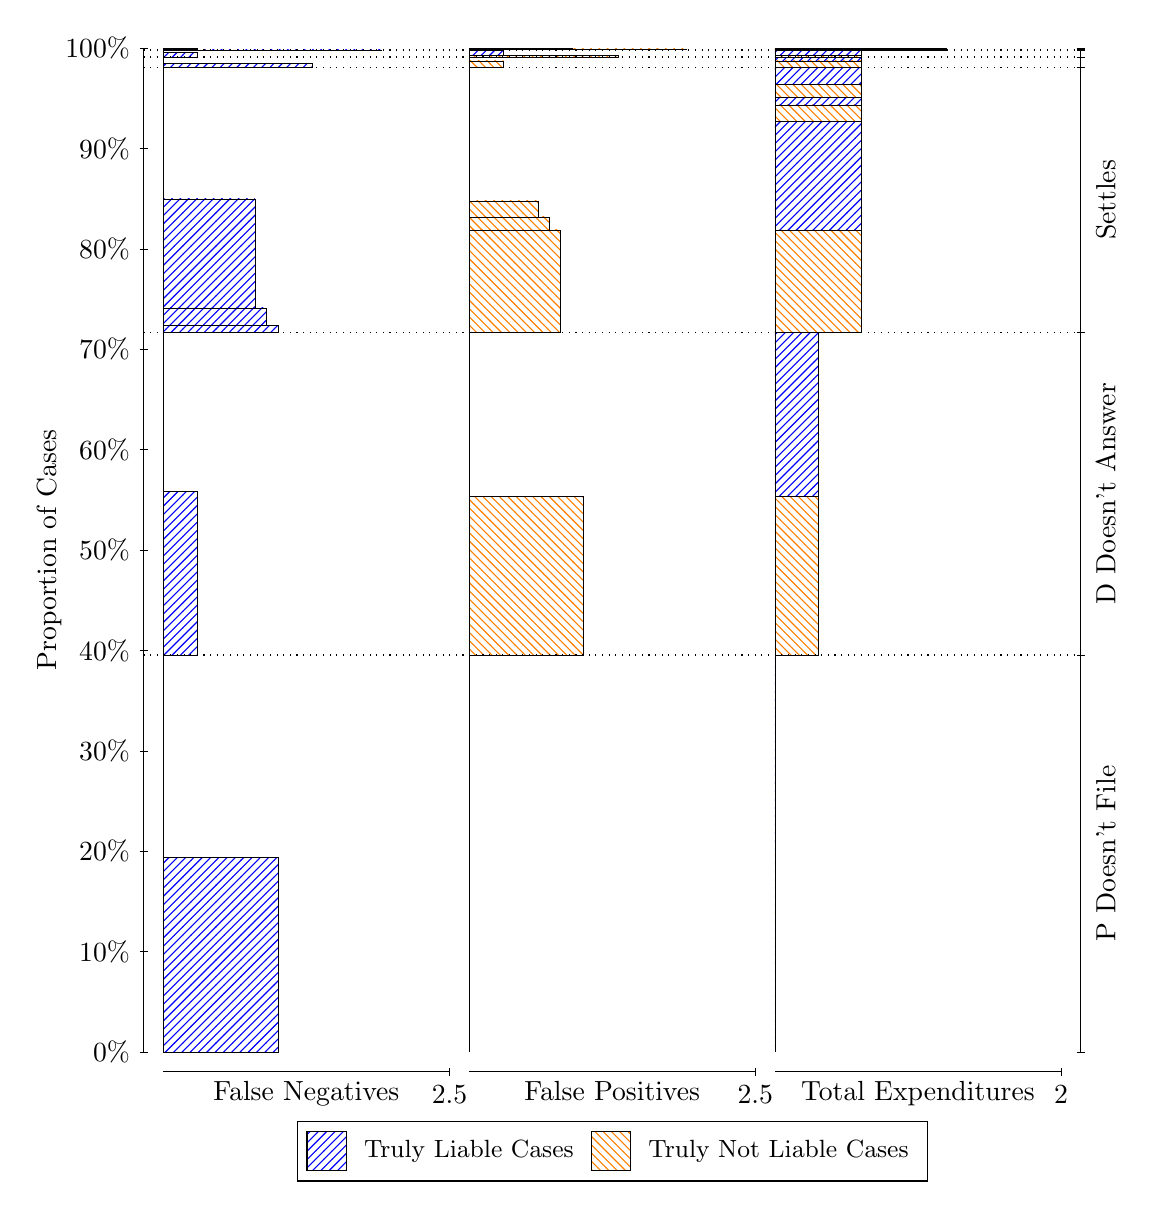
\begin{tikzpicture}
\draw[black, very thin] (1.5,1.75) -- (1.5,14.5);
\node[rotate=90, text=black, anchor=center] at (0.3, 8.125) {Proportion of Cases};
\draw[black, very thin] (1.45,1.75) -- (1.55,1.75);
\node[text=black, anchor=east] at (1.45, 1.75) {0\%};
\draw[black, very thin] (1.45,3.025) -- (1.55,3.025);
\node[text=black, anchor=east] at (1.45, 3.025) {10\%};
\draw[black, very thin] (1.45,4.3) -- (1.55,4.3);
\node[text=black, anchor=east] at (1.45, 4.3) {20\%};
\draw[black, very thin] (1.45,5.575) -- (1.55,5.575);
\node[text=black, anchor=east] at (1.45, 5.575) {30\%};
\draw[black, very thin] (1.45,6.85) -- (1.55,6.85);
\node[text=black, anchor=east] at (1.45, 6.85) {40\%};
\draw[black, very thin] (1.45,8.125) -- (1.55,8.125);
\node[text=black, anchor=east] at (1.45, 8.125) {50\%};
\draw[black, very thin] (1.45,9.4) -- (1.55,9.4);
\node[text=black, anchor=east] at (1.45, 9.4) {60\%};
\draw[black, very thin] (1.45,10.675) -- (1.55,10.675);
\node[text=black, anchor=east] at (1.45, 10.675) {70\%};
\draw[black, very thin] (1.45,11.95) -- (1.55,11.95);
\node[text=black, anchor=east] at (1.45, 11.95) {80\%};
\draw[black, very thin] (1.45,13.225) -- (1.55,13.225);
\node[text=black, anchor=east] at (1.45, 13.225) {90\%};
\draw[black, very thin] (1.45,14.5) -- (1.55,14.5);
\node[text=black, anchor=east] at (1.45, 14.5) {100\%};

\draw[black, very thin] (13.4,1.75) -- (13.4,14.5);
\draw[black, very thin] (13.35,1.75) -- (13.45,1.75);
\node[anchor=west] at (13.35, 1.75) {};
\draw[black, very thin] (13.35,6.7922) -- (13.45,6.7922);
\node[anchor=west] at (13.35, 6.7922) {};
\draw[black, very thin] (13.35,10.884) -- (13.45,10.884);
\node[anchor=west] at (13.35, 10.884) {};
\draw[black, very thin] (13.35,14.258) -- (13.45,14.258);
\node[anchor=west] at (13.35, 14.258) {};
\draw[black, very thin] (13.35,14.386) -- (13.45,14.386);
\node[anchor=west] at (13.35, 14.386) {};
\draw[black, very thin] (13.35,14.47) -- (13.45,14.47);
\node[anchor=west] at (13.35, 14.47) {};
\draw[black, very thin] (13.35,14.485) -- (13.45,14.485);
\node[anchor=west] at (13.35, 14.485) {};
\draw[black, very thin] (13.35,14.5) -- (13.45,14.5);
\node[anchor=west] at (13.35, 14.5) {};

\draw[black, very thin, pattern color=blue, pattern=north east lines] (1.75,1.75) rectangle (3.2033,4.2249);
\draw[black, very thin, pattern color=orange, pattern=north west lines] (1.75,4.2249) rectangle (1.75,6.7922);
\draw[black, very thin, pattern color=blue, pattern=north east lines] (1.75,6.7922) rectangle (2.186,8.8673);
\draw[black, very thin, pattern color=orange, pattern=north west lines] (1.75,8.8673) rectangle (1.75,10.884);
\draw[black, very thin, pattern color=blue, pattern=north east lines] (1.75,10.884) rectangle (3.2033,10.978);
\draw[black, very thin, pattern color=blue, pattern=north east lines] (1.75,10.978) rectangle (3.058,11.201);
\draw[black, very thin, pattern color=blue, pattern=north east lines] (1.75,11.201) rectangle (2.9127,12.583);
\draw[black, very thin, pattern color=orange, pattern=north west lines] (1.75,12.583) rectangle (1.75,14.258);
\draw[black, very thin, pattern color=blue, pattern=north east lines] (1.75,14.258) rectangle (3.6393,14.307);
\draw[black, very thin, pattern color=orange, pattern=north west lines] (1.75,14.307) rectangle (1.75,14.386);
\draw[black, very thin, pattern color=blue, pattern=north east lines] (1.75,14.386) rectangle (2.186,14.447);
\draw[black, very thin, pattern color=orange, pattern=north west lines] (1.75,14.447) rectangle (1.75,14.47);
\draw[black, very thin, pattern color=blue, pattern=north east lines] (1.75,14.47) rectangle (4.5113,14.476);
\draw[black, very thin, pattern color=orange, pattern=north west lines] (1.75,14.476) rectangle (1.75,14.485);
\draw[black, very thin, pattern color=blue, pattern=north east lines] (1.75,14.485) rectangle (2.186,14.495);
\draw[black, very thin, pattern color=orange, pattern=north west lines] (1.75,14.495) rectangle (1.75,14.5);
\draw[black, very thin, pattern color=orange, pattern=north west lines] (5.6333,1.75) rectangle (5.6333,4.3174);
\draw[black, very thin, pattern color=blue, pattern=north east lines] (5.6333,4.3174) rectangle (5.6333,6.7922);
\draw[black, very thin, pattern color=orange, pattern=north west lines] (5.6333,6.7922) rectangle (7.0867,8.8085);
\draw[black, very thin, pattern color=blue, pattern=north east lines] (5.6333,8.8085) rectangle (5.6333,10.884);
\draw[black, very thin, pattern color=orange, pattern=north west lines] (5.6333,10.884) rectangle (6.796,12.191);
\draw[black, very thin, pattern color=orange, pattern=north west lines] (5.6333,12.191) rectangle (6.6507,12.355);
\draw[black, very thin, pattern color=orange, pattern=north west lines] (5.6333,12.355) rectangle (6.5053,12.559);
\draw[black, very thin, pattern color=blue, pattern=north east lines] (5.6333,12.559) rectangle (5.6333,14.258);
\draw[black, very thin, pattern color=orange, pattern=north west lines] (5.6333,14.258) rectangle (6.0693,14.337);
\draw[black, very thin, pattern color=blue, pattern=north east lines] (5.6333,14.337) rectangle (5.6333,14.386);
\draw[black, very thin, pattern color=orange, pattern=north west lines] (5.6333,14.386) rectangle (7.5227,14.41);
\draw[black, very thin, pattern color=blue, pattern=north east lines] (5.6333,14.41) rectangle (6.0693,14.47);
\draw[black, very thin, pattern color=orange, pattern=north west lines] (5.6333,14.47) rectangle (6.0693,14.479);
\draw[black, very thin, pattern color=blue, pattern=north east lines] (5.6333,14.479) rectangle (5.6333,14.485);
\draw[black, very thin, pattern color=orange, pattern=north west lines] (5.6333,14.485) rectangle (8.3947,14.49);
\draw[black, very thin, pattern color=blue, pattern=north east lines] (5.6333,14.49) rectangle (6.9413,14.5);
\draw[black, very thin, pattern color=orange, pattern=north west lines] (9.5167,1.75) rectangle (9.5167,4.3174);
\draw[black, very thin, pattern color=blue, pattern=north east lines] (9.5167,4.3174) rectangle (9.5167,6.7922);
\draw[black, very thin, pattern color=orange, pattern=north west lines] (9.5167,6.7922) rectangle (10.062,8.8085);
\draw[black, very thin, pattern color=blue, pattern=north east lines] (9.5167,8.8085) rectangle (10.062,10.884);
\draw[black, very thin, pattern color=orange, pattern=north west lines] (9.5167,10.884) rectangle (10.607,12.191);
\draw[black, very thin, pattern color=blue, pattern=north east lines] (9.5167,12.191) rectangle (10.607,13.573);
\draw[black, very thin, pattern color=orange, pattern=north west lines] (9.5167,13.573) rectangle (10.607,13.777);
\draw[black, very thin, pattern color=blue, pattern=north east lines] (9.5167,13.777) rectangle (10.607,13.872);
\draw[black, very thin, pattern color=orange, pattern=north west lines] (9.5167,13.872) rectangle (10.607,14.035);
\draw[black, very thin, pattern color=blue, pattern=north east lines] (9.5167,14.035) rectangle (10.607,14.258);
\draw[black, very thin, pattern color=orange, pattern=north west lines] (9.5167,14.258) rectangle (10.607,14.337);
\draw[black, very thin, pattern color=blue, pattern=north east lines] (9.5167,14.337) rectangle (10.607,14.386);
\draw[black, very thin, pattern color=orange, pattern=north west lines] (9.5167,14.386) rectangle (10.607,14.41);
\draw[black, very thin, pattern color=blue, pattern=north east lines] (9.5167,14.41) rectangle (10.607,14.47);
\draw[black, very thin, pattern color=orange, pattern=north west lines] (9.5167,14.47) rectangle (11.697,14.479);
\draw[black, very thin, pattern color=blue, pattern=north east lines] (9.5167,14.479) rectangle (11.697,14.485);
\draw[black, very thin, pattern color=orange, pattern=north west lines] (9.5167,14.485) rectangle (11.697,14.49);
\draw[black, very thin, pattern color=blue, pattern=north east lines] (9.5167,14.49) rectangle (11.697,14.5);
\draw[black, dotted] (1.5,6.7922) -- (13.4,6.7922);
\draw[black, dotted] (1.5,10.884) -- (13.4,10.884);
\draw[black, dotted] (1.5,14.258) -- (13.4,14.258);
\draw[black, dotted] (1.5,14.386) -- (13.4,14.386);
\draw[black, dotted] (1.5,14.47) -- (13.4,14.47);
\draw[black, dotted] (1.5,14.485) -- (13.4,14.485);
\draw[black, very thin] (1.75,1.5) -- (5.3833,1.5);
\node[text=black, anchor=north] at (3.5667, 1.5) {False Negatives};
\draw[black, very thin] (5.3833,1.45) -- (5.3833,1.55);
\node[text=black, anchor=north] at (5.3833, 1.45) {2.5};

\draw[black, very thin] (5.6333,1.5) -- (9.2667,1.5);
\node[text=black, anchor=north] at (7.45, 1.5) {False Positives};
\draw[black, very thin] (9.2667,1.45) -- (9.2667,1.55);
\node[text=black, anchor=north] at (9.2667, 1.45) {2.5};

\draw[black, very thin] (9.5167,1.5) -- (13.15,1.5);
\node[text=black, anchor=north] at (11.333, 1.5) {Total Expenditures};
\draw[black, very thin] (13.15,1.45) -- (13.15,1.55);
\node[text=black, anchor=north] at (13.15, 1.45) {2};

\node[text=black, centered, rotate=90] at (13.72, 4.2711) {P Doesn't File};
\node[text=black, centered, rotate=90] at (13.72, 8.8379) {D Doesn't Answer};
\node[text=black, centered, rotate=90] at (13.72, 12.571) {Settles};





\draw (7.449999999999999,1.5) node[draw=none] (baseCoordinate) {};
\begin{scope}[align=center]
        \matrix[scale=0.5, draw=black, below=0.5cm of baseCoordinate, nodes={draw}, column sep=0.1cm]{
            \node[rectangle, draw, minimum width=0.5cm, minimum height=0.5cm, pattern color=blue, pattern=north east lines] {}; &
            \node[draw=none, font=\small, text=black] (B) {Truly Liable Cases}; &
            \node[rectangle, draw, minimum width=0.5cm, minimum height=0.5cm, pattern color=orange, pattern=north west lines] {}; &
            \node[draw=none, font=\small, text=black] (B) {Truly Not Liable Cases}; \\
            };
\end{scope}

\end{tikzpicture}
\end{document}